\chapter{Diseño del sistema}

\section{Arquitectura (Modelo C4)}

El diseño arquitectónico de \textit{Graphito} se estructura utilizando el Modelo C4, el cual permite describir el software a través de múltiples niveles de abstracción. Esto proporciona diferentes perspectivas técnicas, desde la visión contextual de las interacciones externas hasta el nivel más profundo de componentes.

\subsection{Nivel 1: Contexto}

El diagrama de contexto ilustra cómo el sistema \textbf{GRAPHITO} se relaciona con sus actores externos. En el centro de la arquitectura, el sistema provee las capacidades de procesamiento y análisis. A su alrededor se ubican: el \textbf{Docente}, quien interactúa para gestionar ejercicios, cargar el código de las entregas y visualizar los reportes; y la \textbf{External LLM API}, que es consultada por la plataforma para generar automáticamente soluciones sintéticas que formarán parte del marco de referencias.

\begin{figure}[H]
    \centering
    % Placeholder sugerido, actualizar con la ruta correcta si es diferente 
    
\includegraphics[width=1\textwidth]{figuras/diagrama_contexto.png}
    \caption{Diagrama de Contexto (Nivel 1) del sistema Graphito.}
    \label{fig:c4_contexto}
\end{figure}

\subsection{Nivel 2: Contenedores}

En este nivel de abstracción se detalla la arquitectura de micro-servicios y bases de datos que componen el sistema. \textit{Graphito} se separa funcionalmente en los siguientes contenedores principales:

\begin{itemize}
    \item \textbf{Capa de Cliente (Front-end):} Interfaz web interactiva en \textit{React} que consume servicios REST, facilitando el trabajo del docente.
    \item \textbf{Núcleo de Aplicación (Back-end):} Servicio principal implementado en \textit{FastAPI} (Python) encargado de orquestar el sistema, gestionar las peticiones a la IA y procesar la lógica general.
    \item \textbf{DB Relacional (PostgreSQL):} Persistencia estructurada para datos del usuario, problemas y registro histórico integral del análisis.
    \item \textbf{Vector DB (ChromaDB):} Persistencia hiperdimensional de los \textit{embeddings} que agilizan las búsquedas por proximidad semántica en las referencias.
\end{itemize}

\begin{figure}[H]
    \centering
    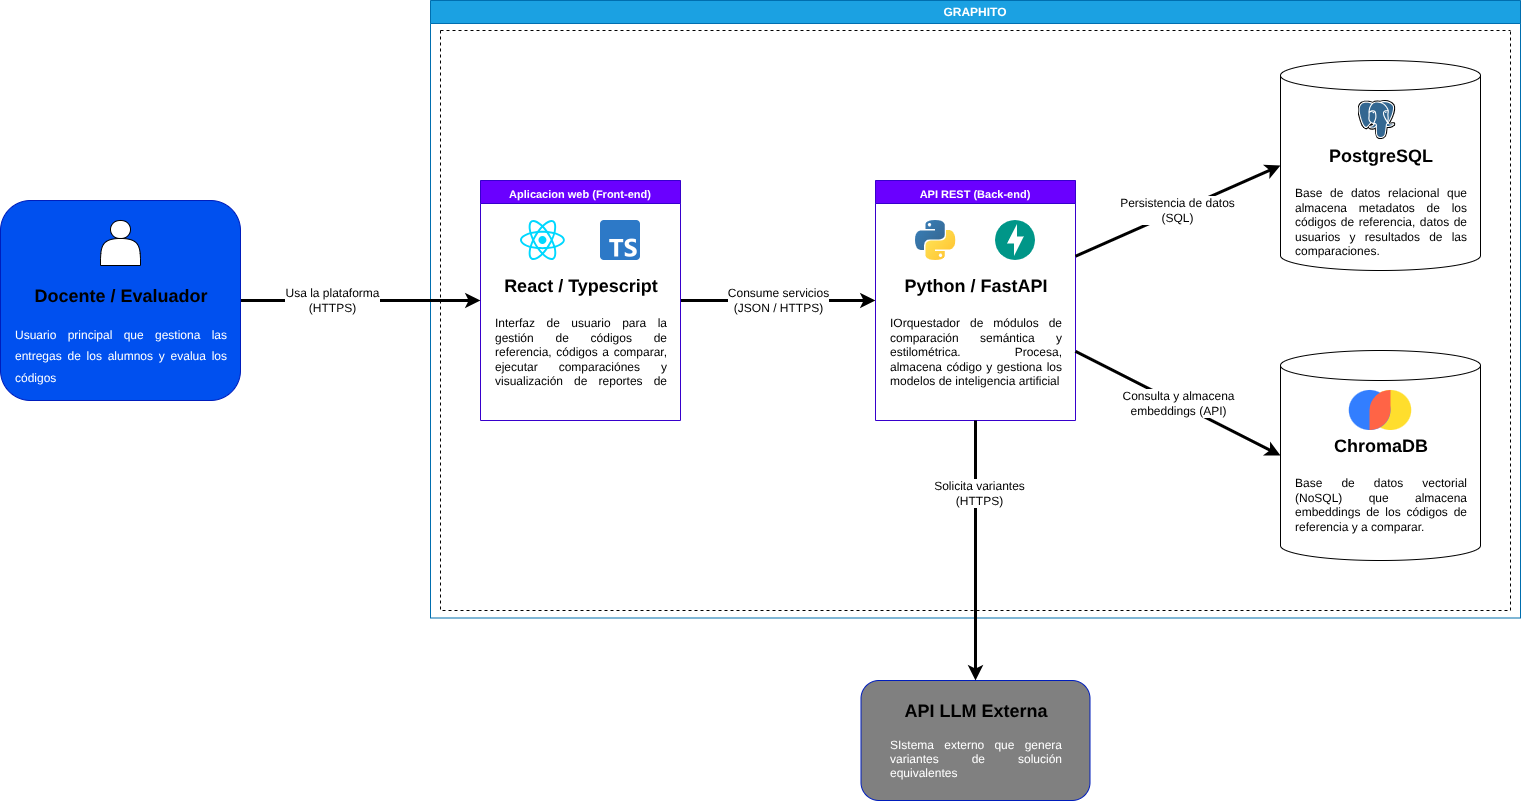
\includegraphics[width=1.0\textwidth]{figuras/diagrama_contenedores.png}
    \caption{Diagrama de Contenedores (Nivel 2) del sistema Graphito.}
    \label{fig:c4_contenedores}
\end{figure}

\subsection{Nivel 3: Componentes}

Haciendo un acercamiento al motor central de analítica del sistema (el contenedor Back-end de FastAPI), se ilustran los componentes internos que materializan la funcionalidad bimodal de auditoría académica para Graphito:

\begin{itemize}
    \item \textbf{Orquestador Inteligente (LangGraph):} Componente maestro de orquestación que evalúa iteraciones, fusiona características biomodales e interactúa cíclicamente para extender las referencias funcionales.
    \item \textbf{Módulo de Análisis Semántico:} Utiliza de forma profunda el modelo pre-entrenado \textit{GraphCodeBERT} para interpretar características lógicas a través del grafo de flujo de datos (DFG).
    \item \textbf{Módulo de Estilometría:} Implementa un clasificador \textit{CharCNN} a nivel de caracteres, capaz de categorizar autorías al aprender la textura de redacción original y capturar singularidades estructurales como sangrías o estilo de corchetes.
\end{itemize}

\begin{figure}[H]
    \centering
    % Placeholder sugerido
    %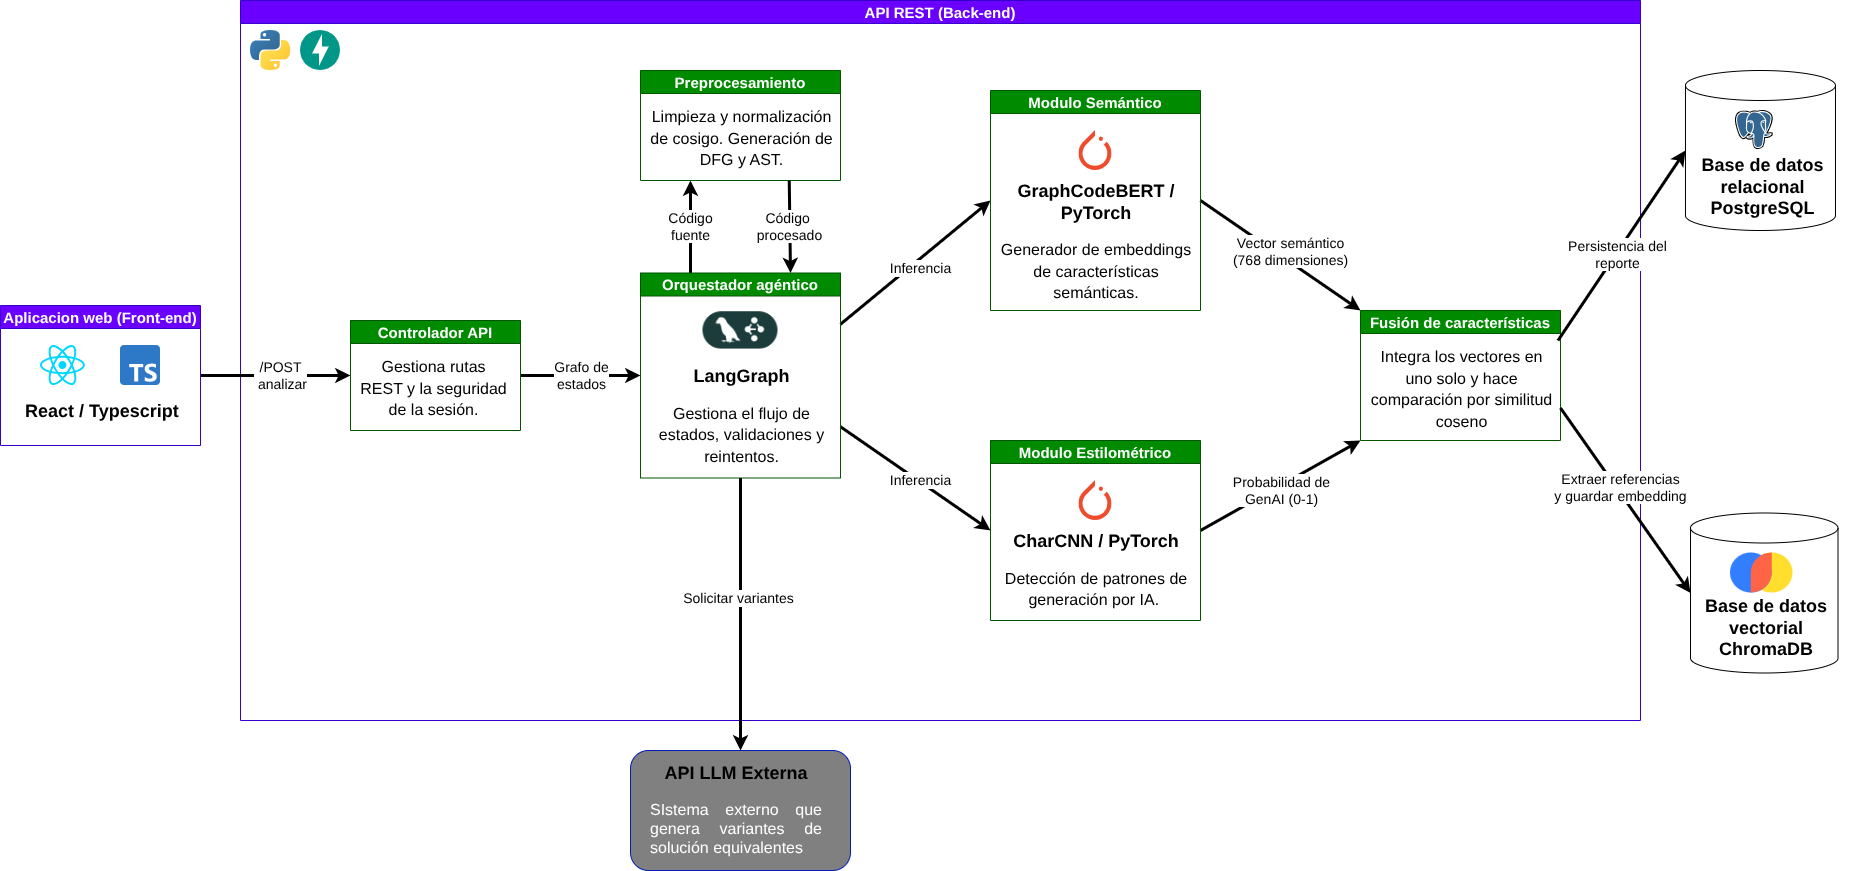
\includegraphics[width=0.8\textwidth]{figuras/diagrama_componentes.png}
    \caption{Diagrama de Componentes (Nivel 3) enfocado en el motor back-end en Python.}
    \label{fig:c4_componentes}
\end{figure}

\subsection{Nivel 4: Código (Clases y Secuencia)}

El nivel de código ofrece el máximo detalle referencial. Se subdivide en la vista estática, representada por las clases y patrones, y la vista dinámica, que muestra el paso a paso transaccional.

\subsubsection{Diagrama de Clases}

A nivel estático, el corazón del diseño obedece al patrón de diseño \textit{Strategy}. 

Como es posible constatar en el la Figura \ref{fig:diagrama_clases_graphito}, la ejecución transaccional principal se centraliza en \textbf{OrquestadorGraphito}, que coordina los módulos. El patrón \textit{Strategy} se aplica a la interfaz de inyección \textbf{ModeloIA}, separando los modelos predictivos como \textbf{ModeloGraphCodeBERT} y \textbf{ModeloCharCNN} del núcleo aplicativo. 

El componente \textbf{Preprocesador} bifurca el ciclo para proveer textos pulidos (análisis semántico) o crudos (estilométrico). Finalizada la ejecución iterativa, se concreta la \textbf{FirmaBimodal}. Por su parte, la persistencia se expone con la interfaz \textbf{AlmacenamientoDatos} la cual rige las lógicas independientes de \textbf{GestorPostgreSQL} y \textbf{GestorChromaDB}.

\begin{figure}[H]
    \centering
    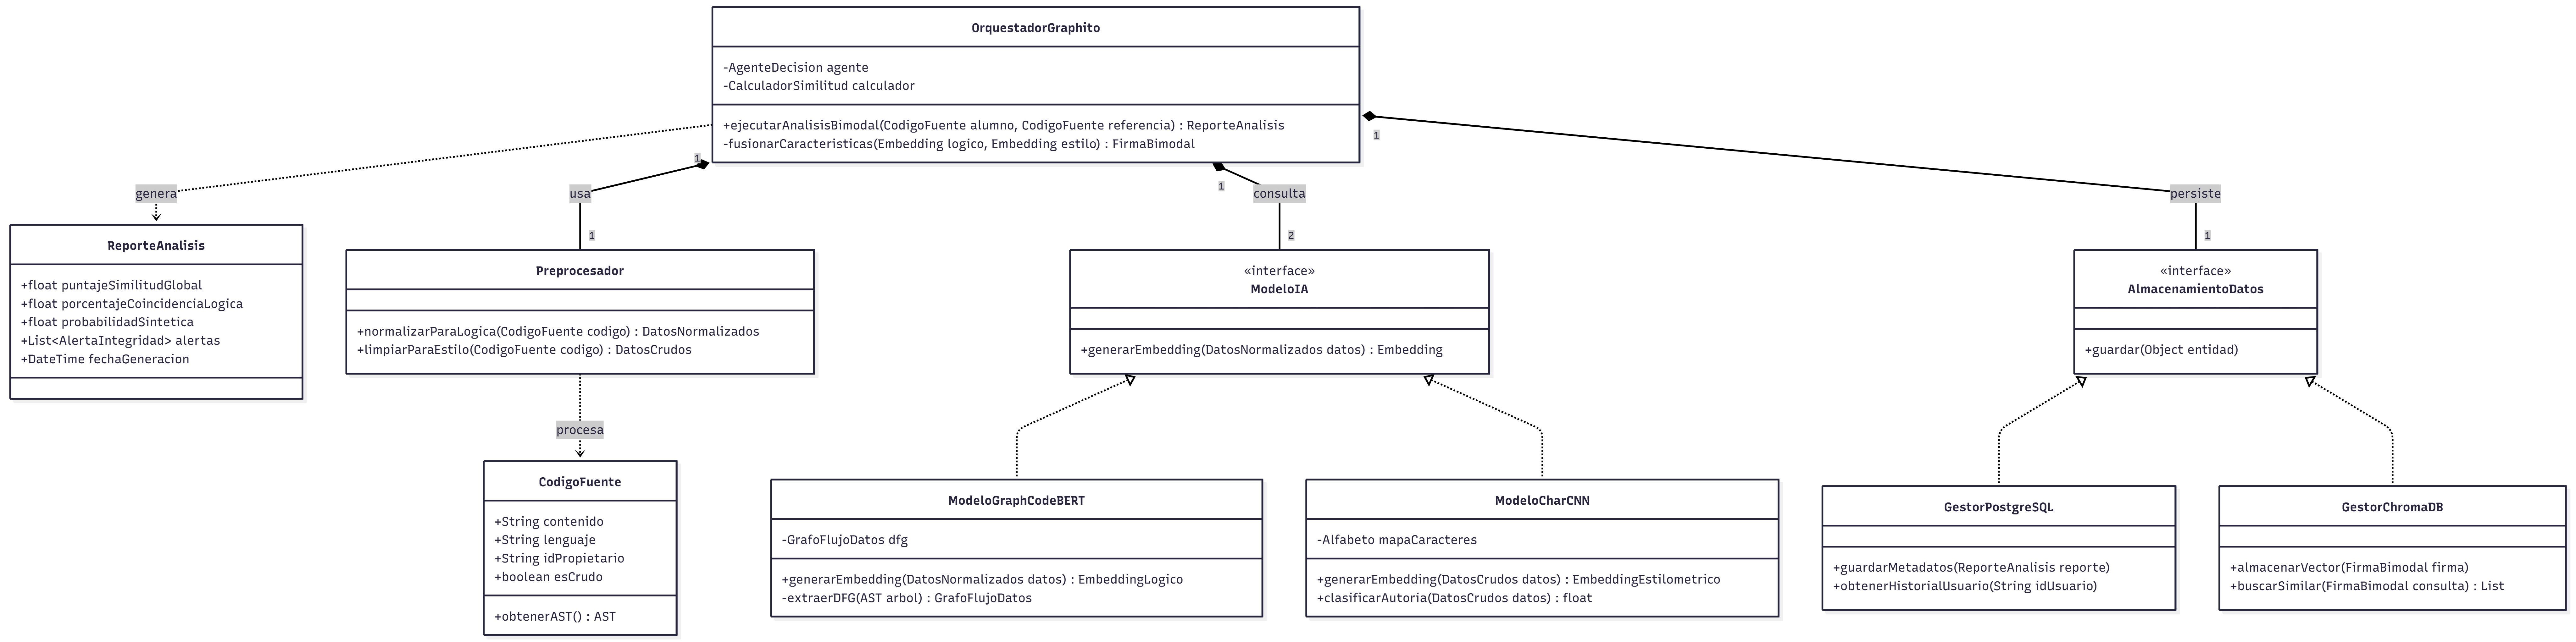
\includegraphics[width=\textwidth]{figuras/diagramaclases.png}
    \caption{Diagrama de clases del sistema Graphito, ilustrando la arquitectura orientada a objetos correspondientes al Nivel 4 de abstracción.}
    \label{fig:diagrama_clases_graphito}
\end{figure}

\subsubsection{Diagrama de Secuencia}

Para el flujo de eventos, el diagrama de secuencia dicta el actuar de los módulos durante una validación estándar:

\begin{itemize}
    \item \textbf{Ejecución Paralela:} Tanto GraphCodeBERT (para entender lógica) como CharCNN (para captar el perfil estilométrico) se ejecutan de manera concurrente con la finalidad de optimizar la inferencia. 
    \item \textbf{Veredicto y Alertas:} Una vez concatenado (\textit{early fusion}) el vector bimodal, se compara su similitud de coseno contra referencias maestras en ChromaDB y, bajo métricas específicas, se retornan las anomalías visuales a la capa de abstracción del frontend.
\end{itemize}

\begin{figure}[H]
    \centering
    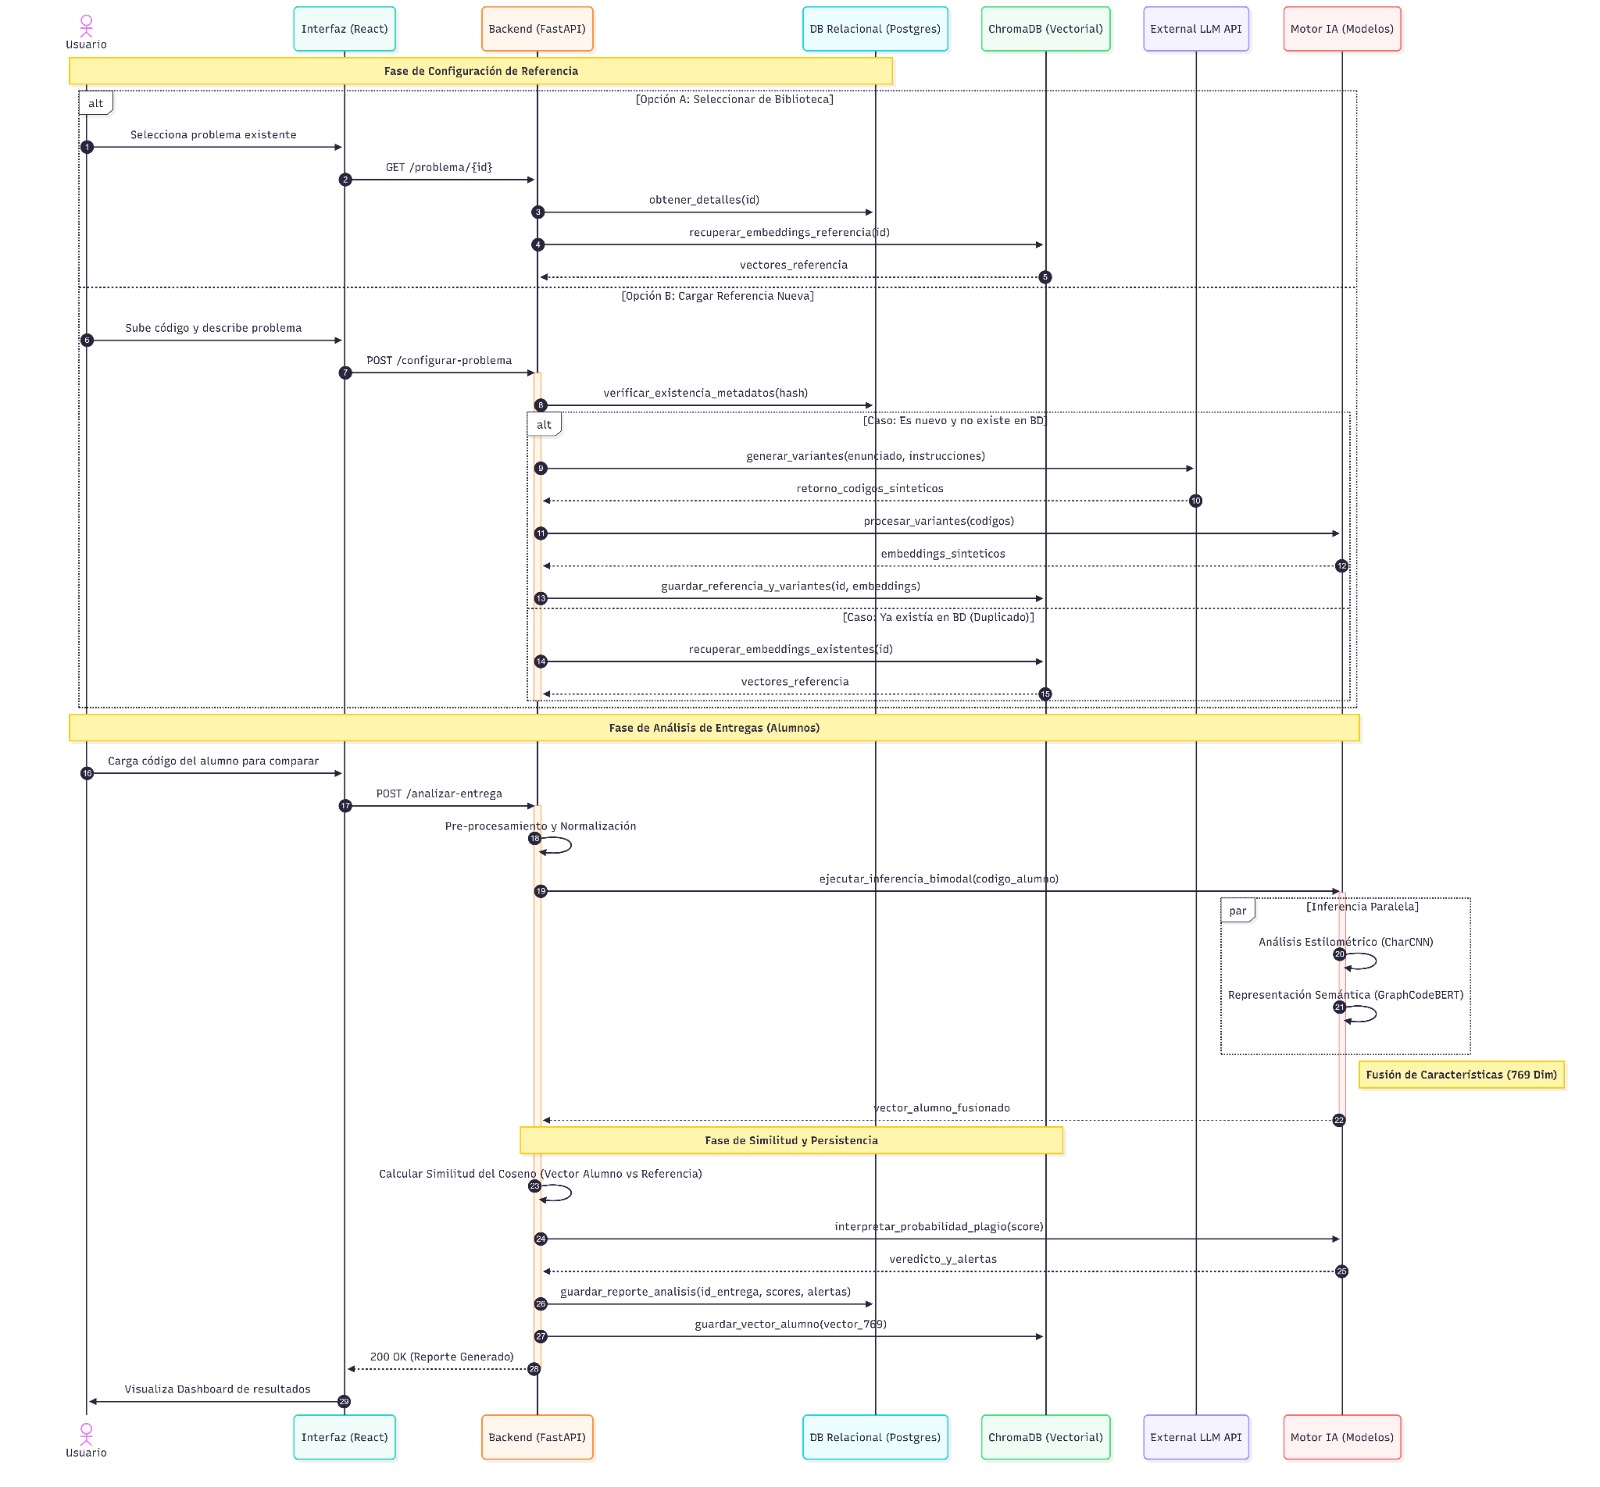
\includegraphics[width=0.9\textwidth]{figuras/diagramaSecuencia.jpeg}
    \caption{Diagrama de secuencia transaccional de \textit{Graphito} desde el cliente, Nivel 4.}
    \label{fig:diagrama_secuencia}
\end{figure}

% ---------------------------------------------------------
\section{Diseño de Base de Datos}
% ---------------------------------------------------------

Se ha implementado un sistema multi-persistencia (relacional y vectorial) para satisfacer requerimientos históricos y heurísticos.

\subsection{Modelo Relacional (Diagrama Entidad-Relación)}

El repositorio SQL maneja registros normalizados con PostgreSQL. Cada \textbf{DOCENTE} gestiona su entidad \textbf{PROBLEMA}. Dicha tabla posee cardinalidad con múltiples instancias de \textbf{CODIGO\_FUENTE} que documentan la entrega cruda en texto o las referencias de origen LLM y su metadata. 

Las similitudes y probabilidades resultantes tienen su hogar en la tabla transaccional \textbf{REPORTE\_ANALISIS}, la cual desencadena notificaciones a la entidad de \textbf{ALERTA\_INTEGRIDAD} al identificar comportamientos fuera del límite permisible en términos de completitud lógica versus artificialidad de estilo.

\begin{figure}[H]
    \centering
    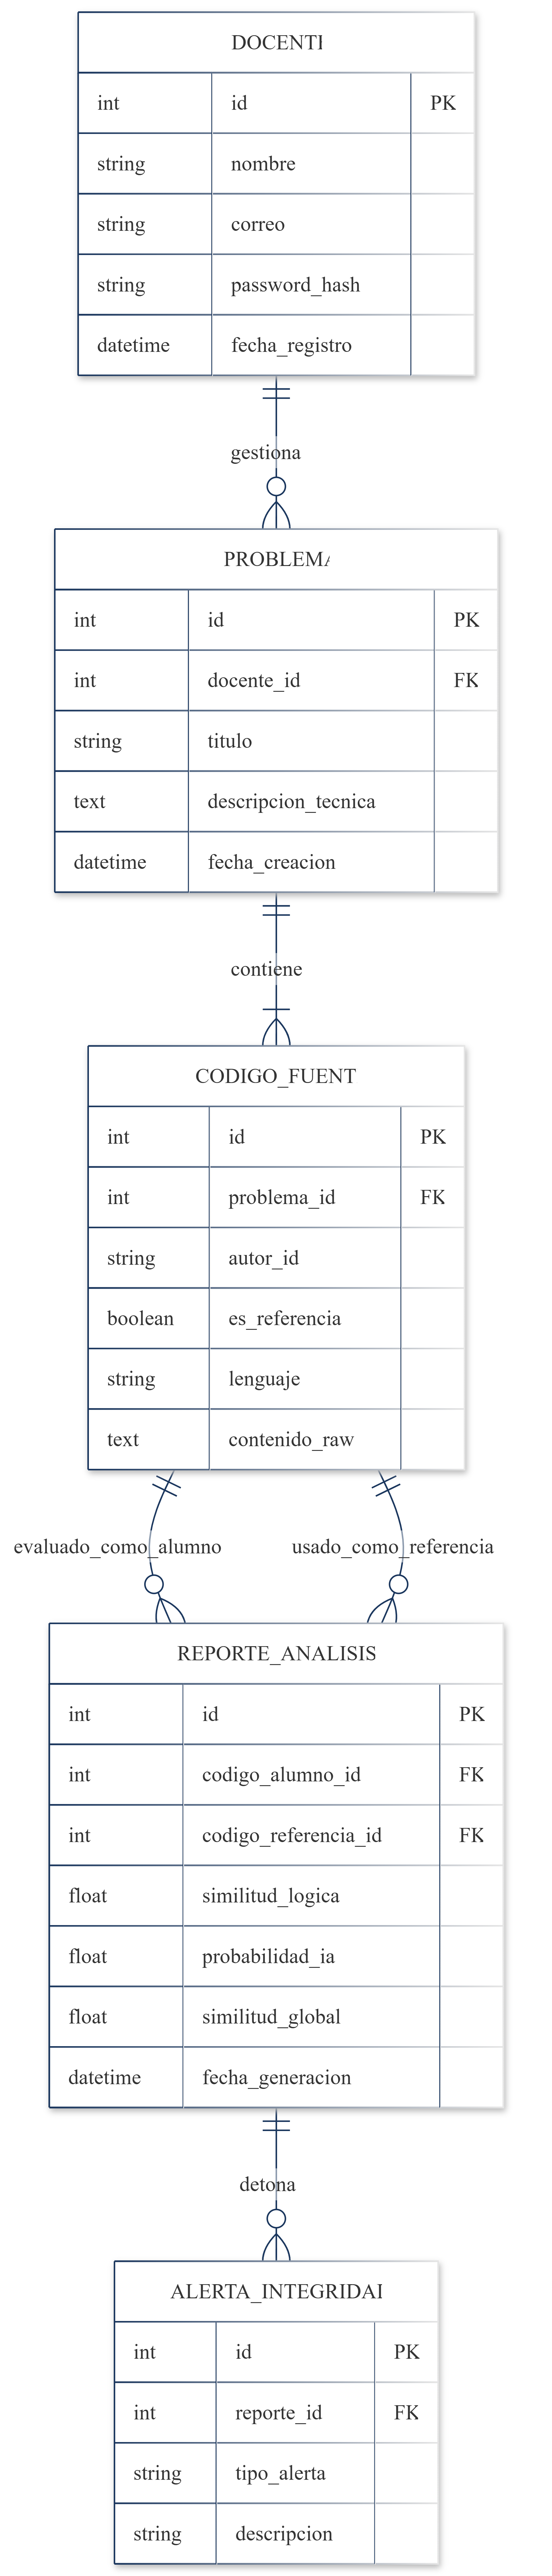
\includegraphics[width=\textwidth, height=0.75\textheight, keepaspectratio]{figuras/diagramarelacional.png}
    \caption{Diagrama C4 y Entidad-Relación de PostgreSQL sobre el componente integrador.}
    \label{fig:diagrama_er_graphito}
\end{figure}

\subsection{Esquema de Colección Vectorial (ChromaDB)}

La persistencia heurística se hospeda en el clúster transitorio o indexado de ChromaDB. Se estipuló un indexado central mediante la colección denominada \texttt{codigos\_referencia}, empleando UUIDs que coinciden con los registros almacenados en \texttt{CODIGO\_FUENTE} de su contraparte relacional.

Esta base vectorial aloja un \textit{embedding híbrido o concatenado} compuesto exactamente por \textbf{769 dimensiones}:
\begin{enumerate}
    \item \textbf{Dimensión [0 a 767] (Semántica):} Son formadas íntegramente por \textit{GraphCodeBERT} abstrayendo el comportamiento funcional del código.
    \item \textbf{Dimensión [768] (Estilometría):} Valor predictivo escalar inyectado desde la matriz \textit{CharCNN} donde se penaliza matemáticamente la autenticidad cuando los trazos reflejan una estructura sintética LLM.
\end{enumerate}

Para acelerar la segmentación del análisis de referencias, todos los nodos dentro de la colección ChromaDB se engloban con metadatos JSON básicos conteniendo al identificador de lógica (\texttt{problema\_id}), marcadores booleanos (\texttt{es\_referencia}), el ecosistema matriz como (\texttt{lenguaje}: \texttt{C|C++}) y un catalogador simple (\texttt{author\_type}).

% ---------------------------------------------------------
\section{Maquetación de la Interfaz}
% ---------------------------------------------------------

Para validar el análisis y diseño propuestos, se desarrollaron diferentes interfaces y componentes que conforman el prototipo inicial del sistema Graphito. A continuación, se documentan dichas pantallas, estableciendo la relación entre las vistas del sistema y los requerimientos funcionales definidos previamente.

\subsection{Arquitectura de Información}
La arquitectura de información del prototipo ha sido planteada para mantener un flujo intuitivo en la labor del docente. El sistema se compone de un área pública para la autenticación, y un área privada o "Centro de Mando" desde donde el usuario puede gestionar sus ejercicios, subir nuevas entregas y examinar los resultados del análisis semántico y estilométrico. Se prioriza una navegación jerárquica sencilla, facilitando el acceso a los reportes y comparaciones detalladas.

\subsection{Diseño de Interfaces (Pantallas)}

El diseño visual y funcional del prototipo aborda las principales necesidades del evaluador. A continuación, se presentan las diversas pantallas implementadas que demuestran el cumplimiento de los requerimientos de la plataforma.

\subsubsection{Inicio de Sesión y Registro}
El sistema cuenta con un área pública que permite a los docentes autenticarse y crear una cuenta, asegurando la privacidad de los ejercicios.

\begin{figure}[H]
    \centering
    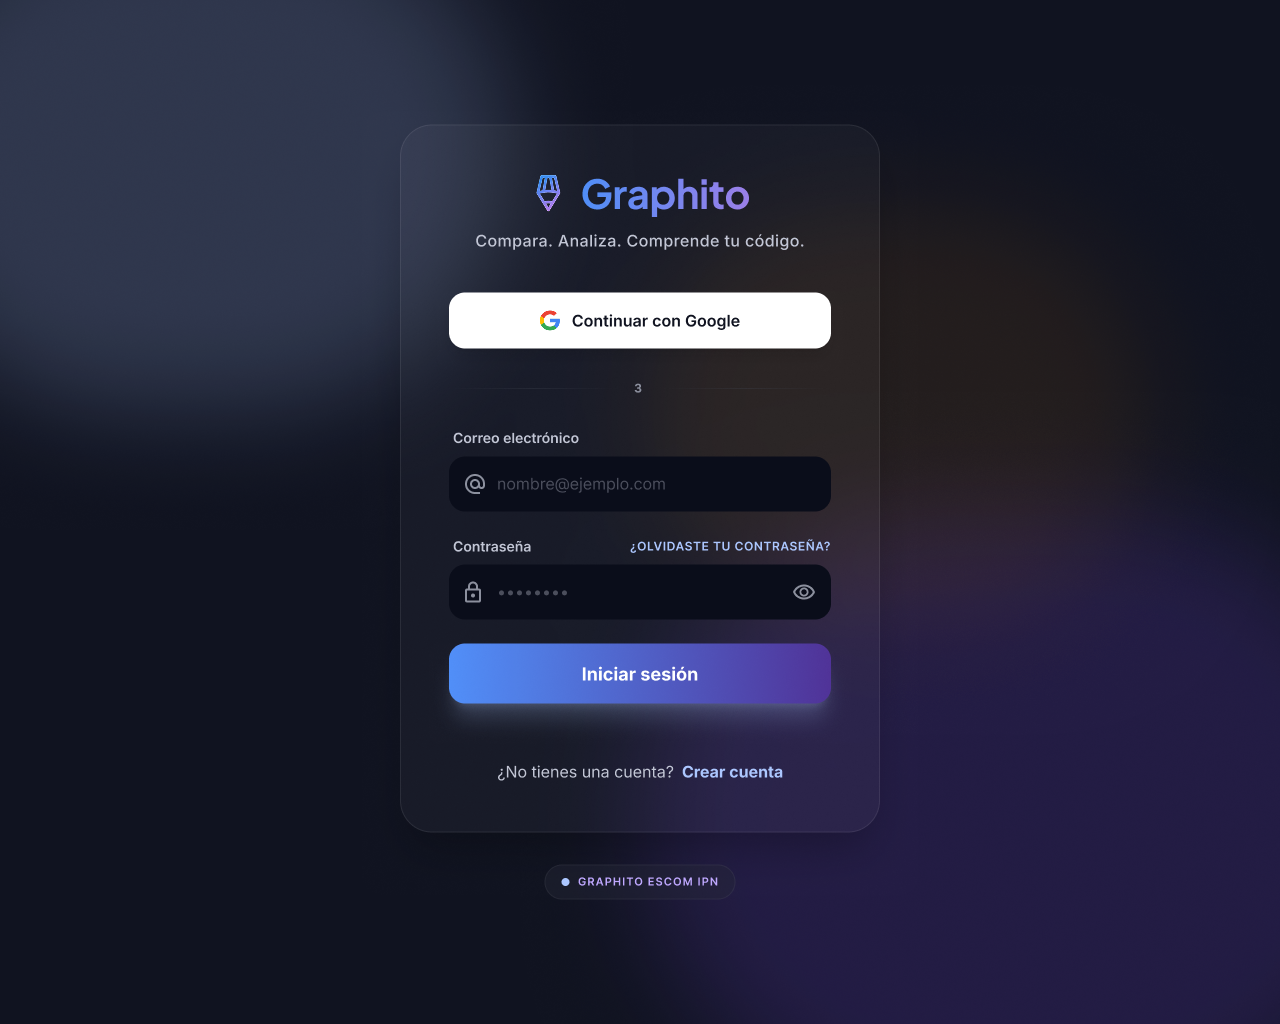
\includegraphics[width=0.8\textwidth]{figuras/iniciar_sesión.png}
    \caption{Interfaz de inicio de sesión, cumpliendo con el RF-01.}
    \label{fig:ui_iniciar_sesion}
\end{figure}

\begin{figure}[H]
    \centering
    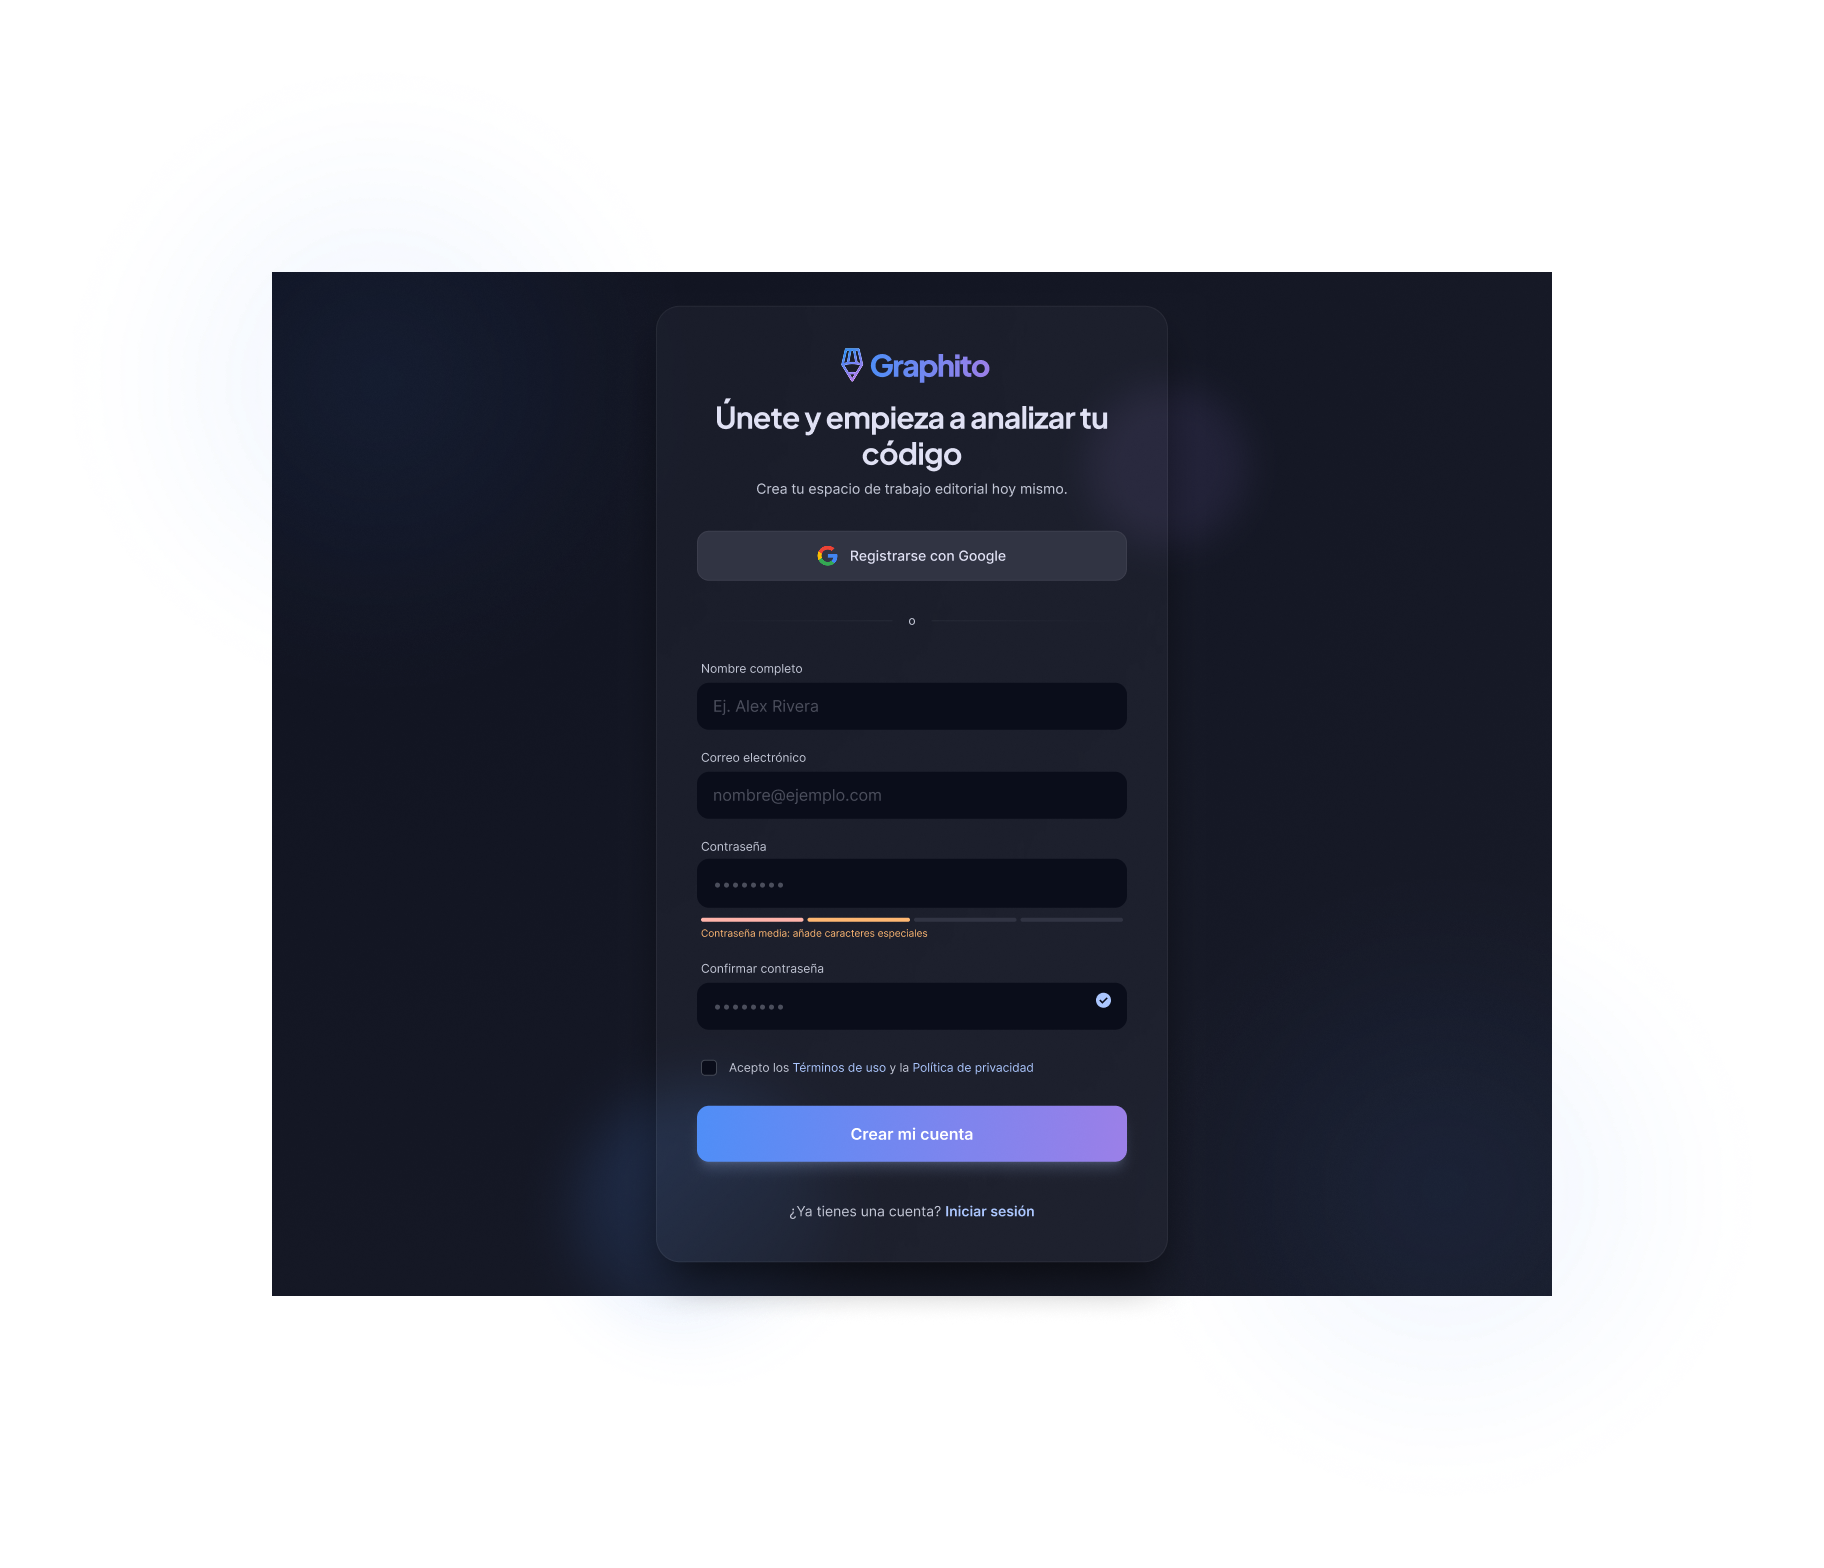
\includegraphics[width=0.8\textwidth]{figuras/crear_cuenta.png}
    \caption{Interfaz de creación de cuenta.}
    \label{fig:ui_crear_cuenta}
\end{figure}

\subsubsection{Interfaz de Carga de Código}
Se diseñó un mecanismo de carga sencillo para que los docentes integren nuevos archivos al sistema, agreguen comparaciones y comiencen el análisis automático de las entregas.

\begin{figure}[H]
    \centering
    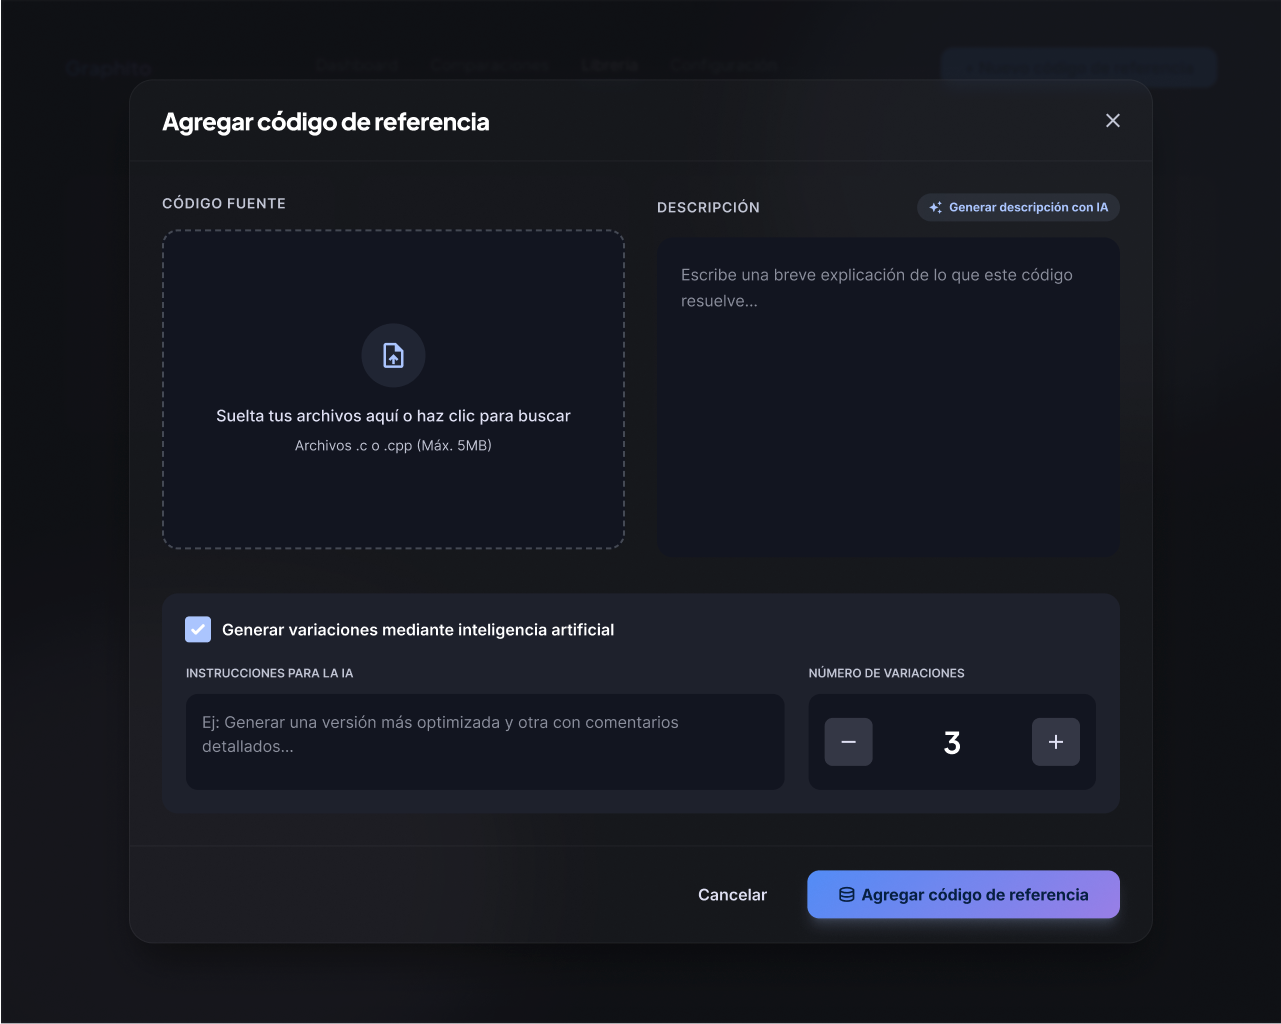
\includegraphics[width=0.8\textwidth]{figuras/nuevo_código_de_referencia.png}
    \caption{Interfaz para nuevo código de referencia, cumpliendo con el RF-03.}
    \label{fig:ui_carga_ref}
\end{figure}

\begin{figure}[H]
    \centering
    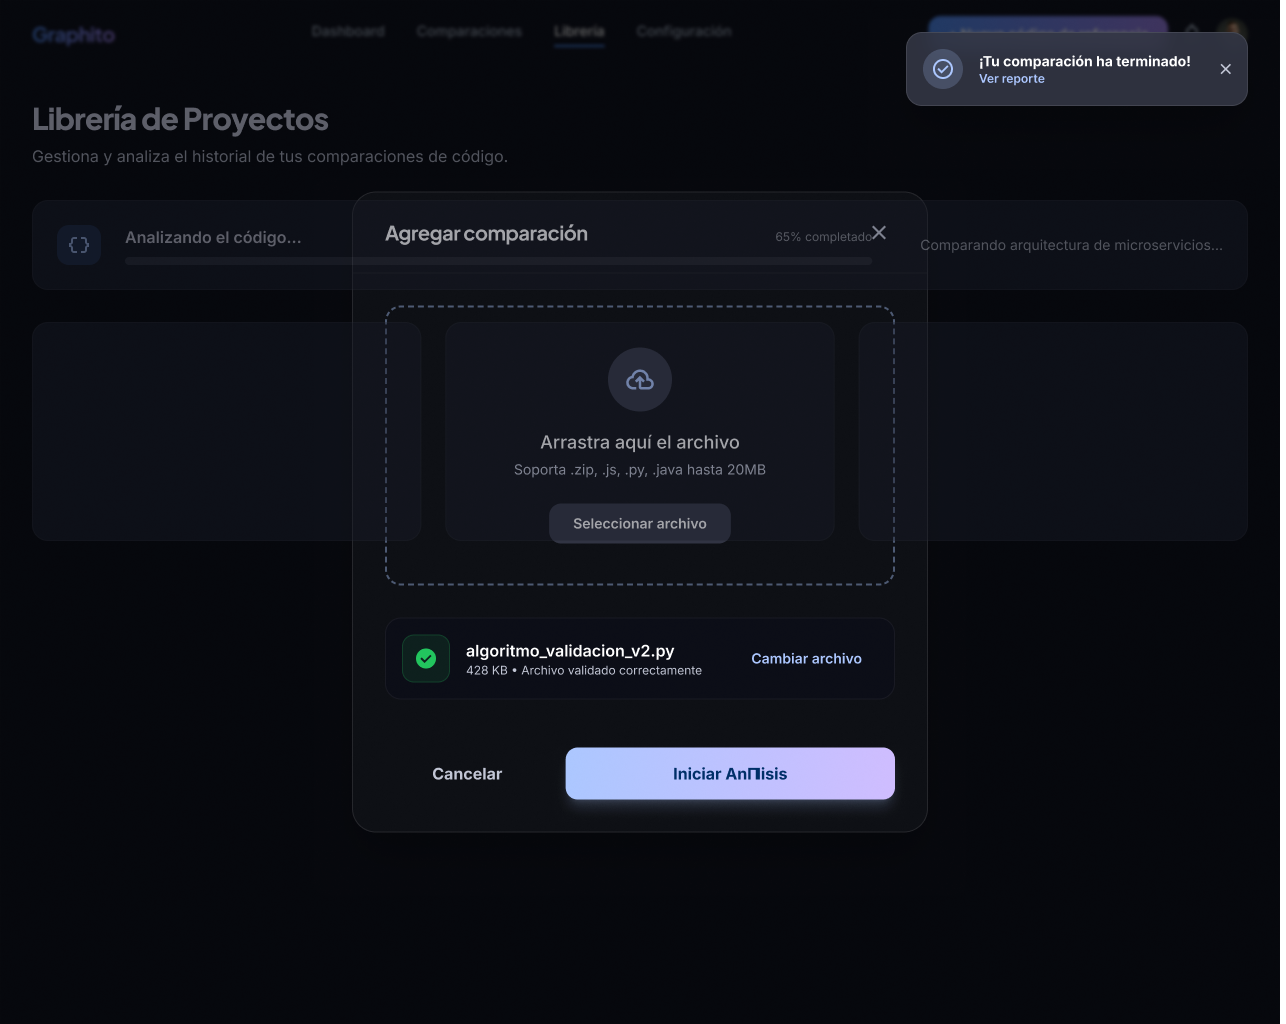
\includegraphics[width=0.8\textwidth]{figuras/agregar_comparación.png}
    \caption{Interfaz para agregar comparación.}
    \label{fig:ui_carga_comp}
\end{figure}

\subsubsection{Interfaz de Gestión y Repositorio}
Para organizar de manera efectiva el trabajo docente, el sistema cuenta con un repositorio personal de ejercicios.

\begin{figure}[H]
    \centering
    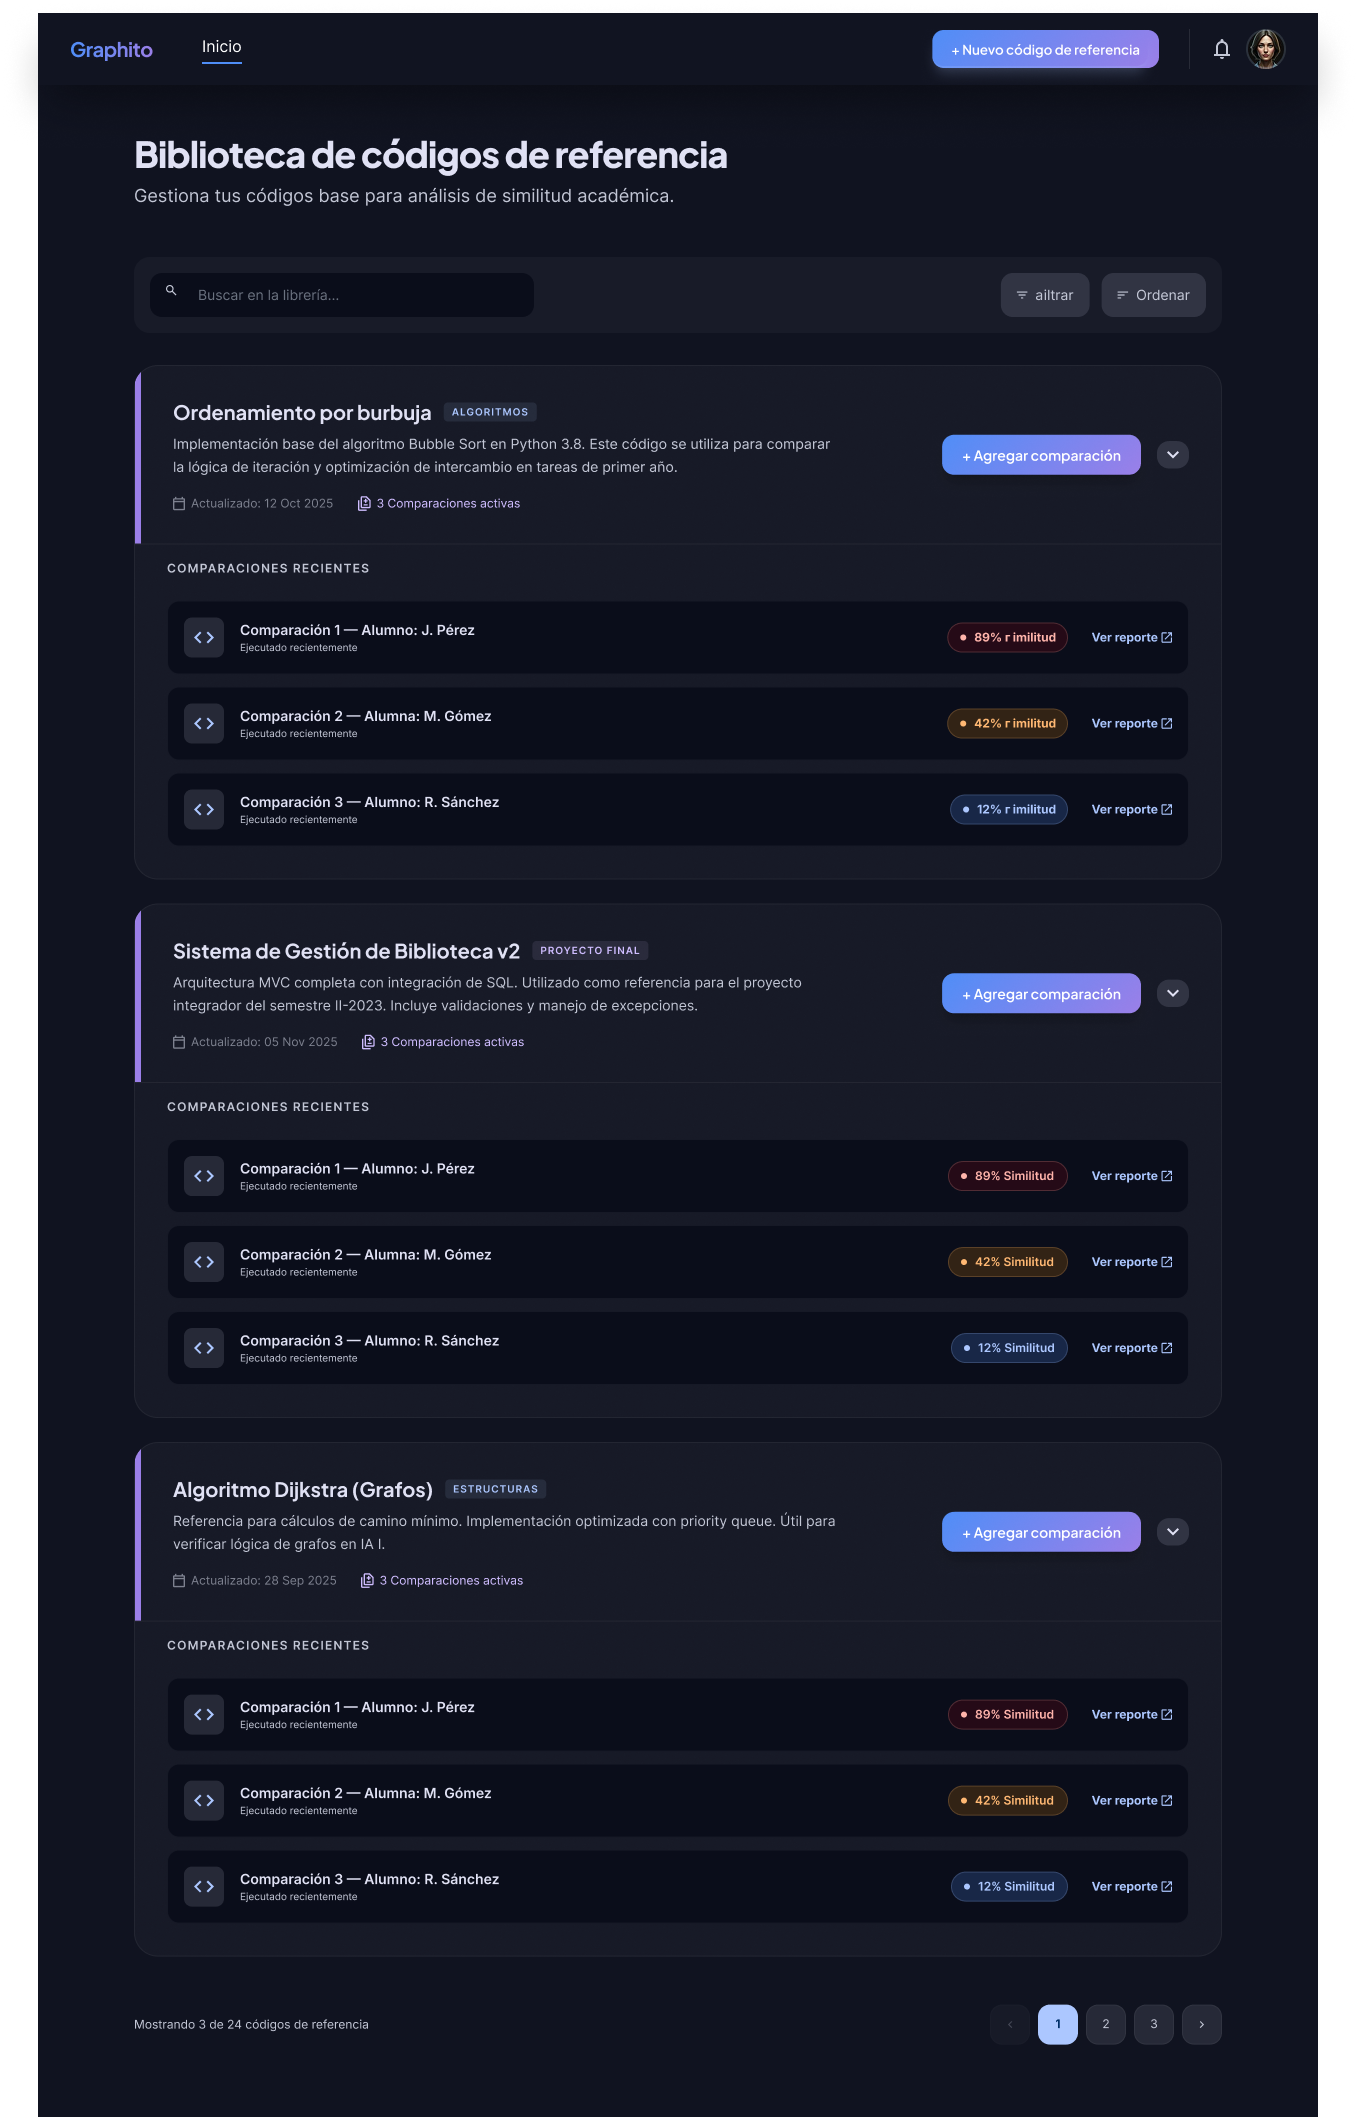
\includegraphics[width=0.8\textwidth]{figuras/biblioteca_de_referencias.png}
    \caption{Repositorio personal de ejercicios, cumpliendo con el RF-02.}
    \label{fig:ui_repositorio}
\end{figure}

El \textbf{RF-02} especifica que el sistema debe permitir al docente la creación y gestión de un listado de ejercicios o problemas de programación. La Figura \ref{fig:ui_repositorio} muestra la implementación de esta funcionalidad, ofreciendo una vista consolidada de los problemas registrados.

\subsubsection{Reporte de Análisis Bimodal}
La pantalla principal de resultados presenta de forma integral las métricas calculadas por los motores de inteligencia artificial.

\begin{figure}[H]
    \centering
    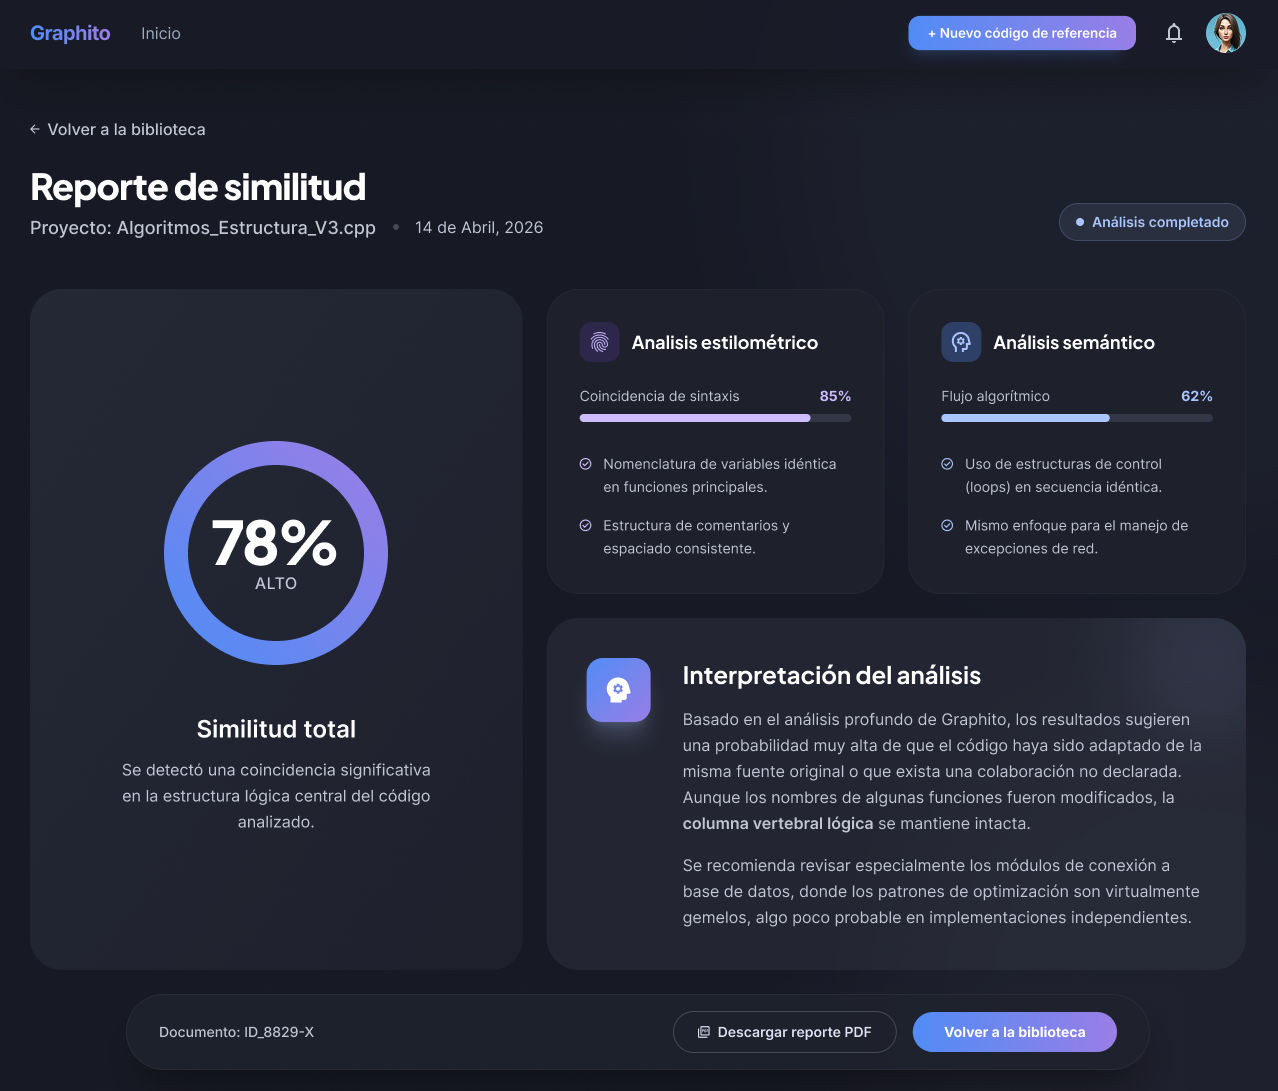
\includegraphics[width=0.8\textwidth]{figuras/reporte_de_similitud.png}
    \caption{Dashboard de reporte bimodal, cumpliendo con el RF-10 y RF-11.}
    \label{fig:ui_reporte}
\end{figure}

En la Figura \ref{fig:ui_reporte} se visualiza la interfaz del reporte, cumpliendo con el \textbf{RF-10} sobre la necesidad de generar un reporte bimodal que integre el índice de similitud semántica y la probabilidad de autoría de forma visual. Además, esta pantalla despliega de manera automática las alertas de integridad estipuladas en el \textbf{RF-11} frente a discrepancias entre la lógica y el estilo.
